\documentclass[12pt,fleqn]{article}\usepackage{../../common}
\begin{document}
Uygulama - Yağmur Yağış Verisi

\begin{minted}[fontsize=\footnotesize]{python}
import pandas as pd
df = pd.read_csv('rainfall.csv',index_col=0,parse_dates=['dt'])
df.columns = ['rain']
\end{minted}

Markov Zinciri hazirligi, onceki gun yagis olup olmadigi D2, iki gun once D1,
bugun D3.

\begin{minted}[fontsize=\footnotesize]{python}
df['r1ago'] = df.rain.shift(1)
df['r2ago'] = df.rain.shift(2)
df['D1'] = df.apply(lambda x: (x.r2ago > 0.0).astype(float), axis=1)
df['D2'] = df.apply(lambda x: (x.r1ago > 0.0).astype(float), axis=1)
df['D3'] = df.apply(lambda x: (x.rain > 0.0).astype(float), axis=1)
pd.set_option('display.max_columns', None)
print (df)
\end{minted}

\begin{verbatim}
            rain  r1ago  r2ago   D1   D2   D3
dt                                           
2015-01-01   0.6    NaN    NaN  0.0  0.0  1.0
2015-01-02   0.0    0.6    NaN  0.0  1.0  0.0
2015-01-03   0.0    0.0    0.6  1.0  0.0  0.0
2015-01-04   0.0    0.0    0.0  0.0  0.0  0.0
2015-01-05   0.0    0.0    0.0  0.0  0.0  0.0
...          ...    ...    ...  ...  ...  ...
2022-01-27   0.0    0.0    0.0  0.0  0.0  0.0
2022-01-28   0.0    0.0    0.0  0.0  0.0  0.0
2022-01-29   0.0    0.0    0.0  0.0  0.0  0.0
2022-01-30   3.8    0.0    0.0  0.0  0.0  1.0
2022-01-31   0.0    3.8    0.0  0.0  1.0  0.0

[2588 rows x 6 columns]
\end{verbatim}


\begin{minted}[fontsize=\footnotesize]{python}
x = df[df.index.month == 3]['rain']
\end{minted}

\begin{minted}[fontsize=\footnotesize]{python}
from scipy.stats import gamma
res = gamma.fit(df['rain'])
a,loc,scale = res  
x.hist(density=True)
plt.ylim(0,0.4)
plt.plot(x, gamma.pdf(x,a,loc,scale),'r.')
plt.savefig('stat_176_app1_01.png')
\end{minted}

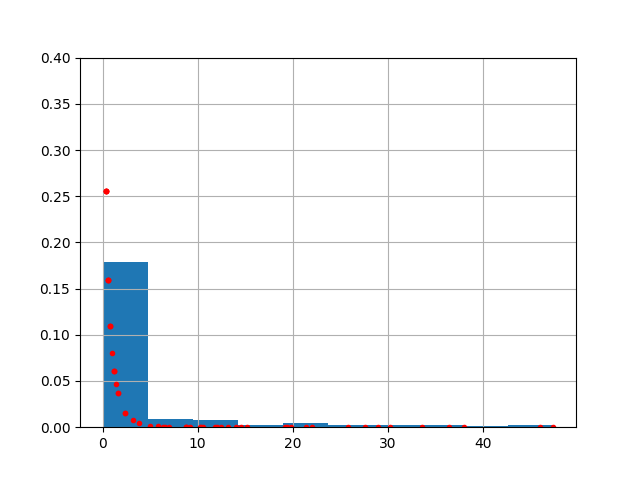
\includegraphics[width=20em]{stat_176_app1_01.png}

Veriye olan uygunluğu kontrol için olasılık dağılımları arasında bir yakınlık
ölçüsü olan Kullback-Leibler mesafesini [2] kullanalım. Veri histogramı ve
tahmin edilen dağılım üzerinden üretilen verinin histogramı arasında mesafeyi
alttaki fonksiyon ile ölçebiliriz,

\begin{minted}[fontsize=\footnotesize]{python}
def kl(p, q):
    return np.sum(p * np.log(p / q))    
\end{minted}

\begin{minted}[fontsize=\footnotesize]{python}
b = range(0,50)
eps = 1e-5
s = 4000
dh = np.histogram(df.rain, bins=b, density=True)[0]+eps

r1 = gamma.rvs(a,loc,scale,size=s)
h1 = np.histogram(r1, bins=b, density=True)[0]+eps
print ('Gamma', kl(h1, dh))
\end{minted}

\begin{verbatim}
Gamma 0.285281002063564
\end{verbatim}

\begin{minted}[fontsize=\footnotesize]{python}
from scipy.stats import weibull_min
res = weibull_min.fit(df['rain'])
a,loc,scale = res  
x.hist(density=True)
plt.ylim(0,0.4)
plt.plot(x, weibull_min.pdf(x,a,loc,scale),'r.')
plt.savefig('stat_176_app1_02.png')
\end{minted}

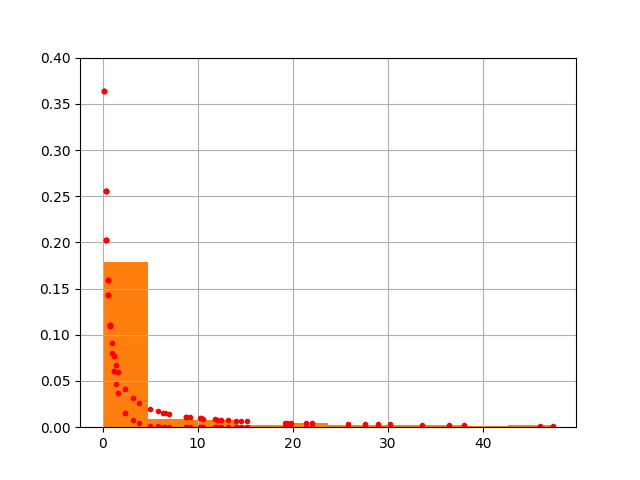
\includegraphics[width=20em]{stat_176_app1_02.png}

\begin{minted}[fontsize=\footnotesize]{python}
r2 = weibull_min.rvs(a,loc,scale,size=s)
h2 = np.histogram(r2, bins=b, density=True)[0]+eps
print ('Weibull Min', kl(h2, dh))
\end{minted}

\begin{verbatim}
Weibull Min 0.06420630403960519
\end{verbatim}

Weibull Min daha yakin gozukuyor.



Kaynaklar

[1] {\em Meteorological Service Singapore},
    \url{http://www.weather.gov.sg/climate-historical-daily/}

[2] Bayramli, {\em Kullback-Leibler (KL) Mesafesi}
    
\end{document}



